\chapter{Конструкторская часть}

В данном разделе представлены схемы алгоритмов конвейерной обработки данных и этапов обработки текста.

\section{Разработка алгоритма приведения слова к начальной форме}
В рамках данной работы не рассматривается алгоритм приведения слова к начальной форме. Реализован алгоритм будет с использованием внешних библиотек.

\section{Разработка алгоритма дедупликации текста}
На рис. \ref{img:alg1} представлена схема алгоритма дедупликации текста.

\begin{figure}[h!]
\centering
    \includegraphics[width=0.75\linewidth]{deduplicate.pdf}
    \caption{Схема алгоритма дедупликации текста}
    \label{img:alg1}	
\end{figure}

\newpage

\section{Разработка алгоритма нахождения частоты терма в тексте}
На рис. \ref{img:alg2} представлена схема алгоритма нахождения частоты терма в тексте.

\begin{figure}[h!]
\centering
    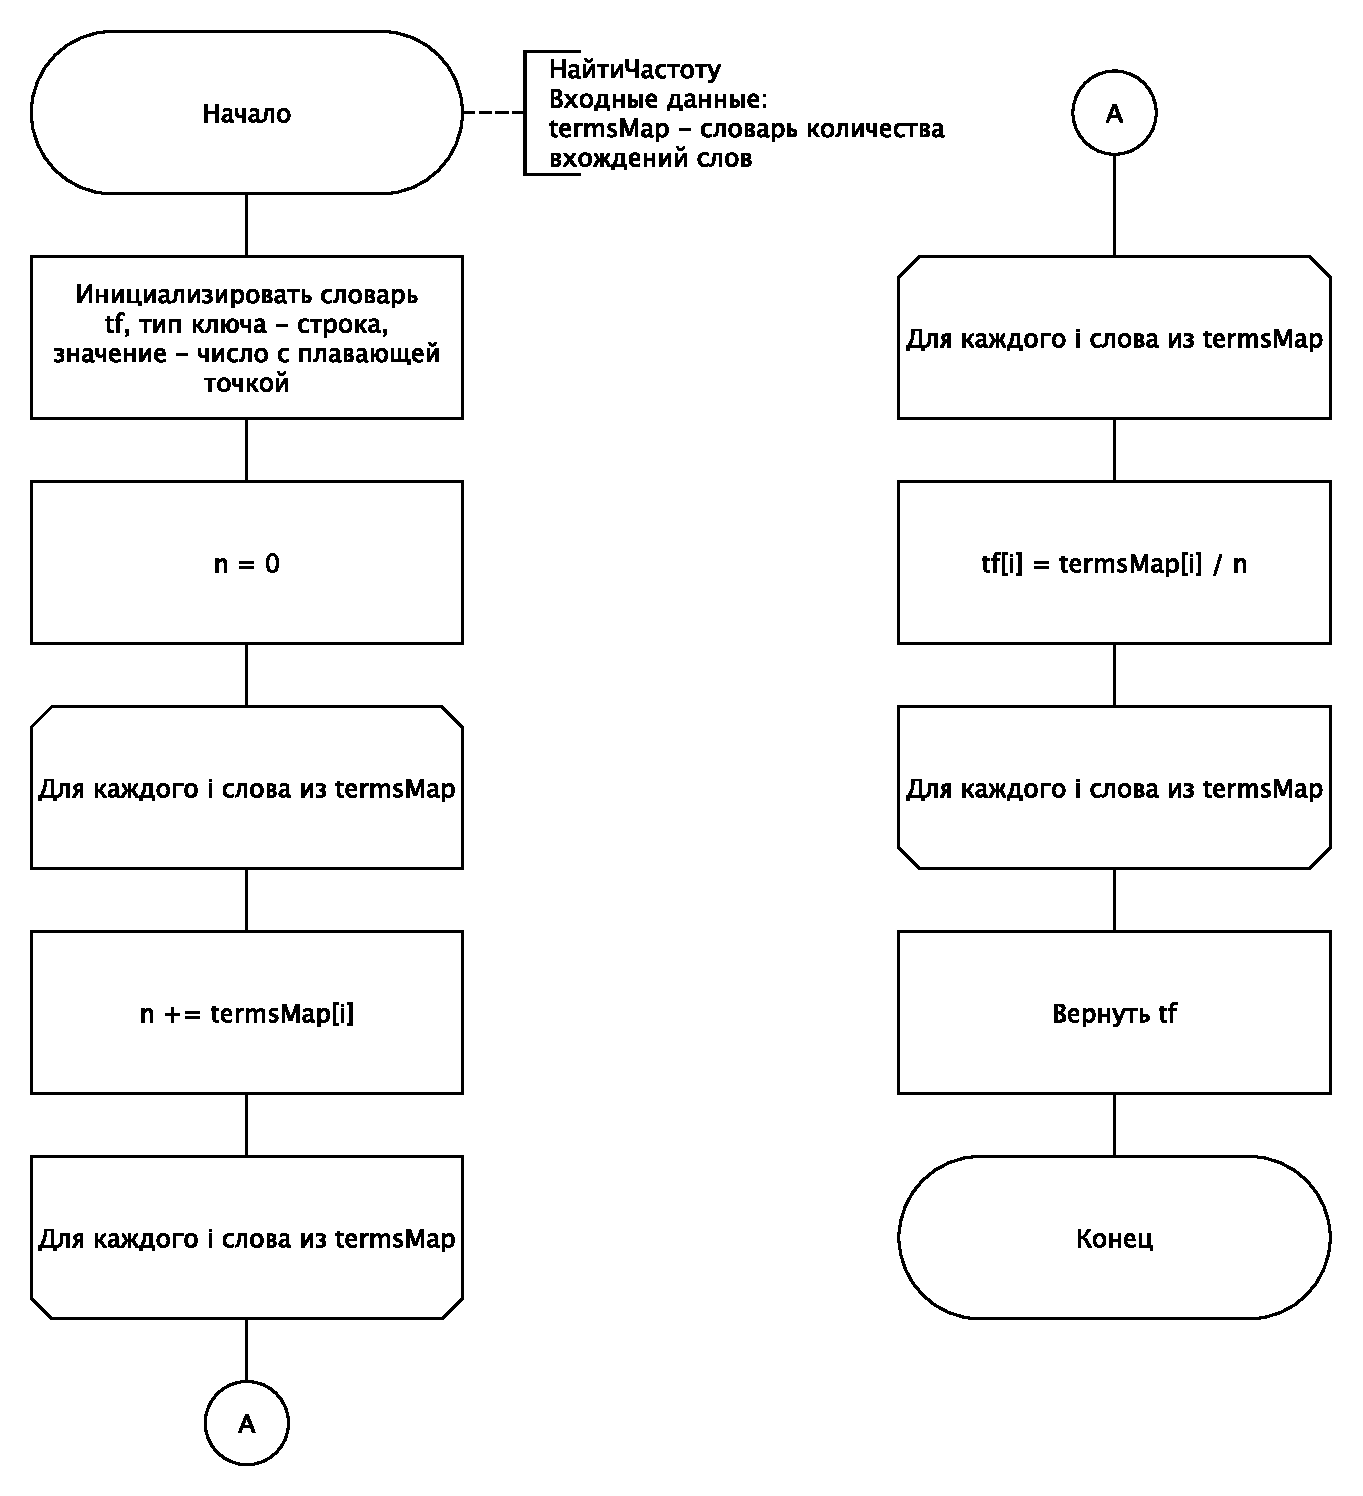
\includegraphics[width=1\linewidth]{tf.pdf}
    \caption{Схема алгоритма нахождения частоты терма в тексте}
    \label{img:alg2}	
\end{figure}

\newpage

\section{Разработка алгоритма последовательной конвейерной обработки текста}
На рис. \ref{img:alg3} представлена схема алгоритма последовательной конвейерной обработки текста.

\begin{figure}[h!]
\centering
    \includegraphics[width=0.85\linewidth]{pipeline_usual.pdf}
    \caption{Схема алгоритма последовательной конвейерной обработки текста}
    \label{img:alg3}	
\end{figure}

\newpage

\section{Разработка алгоритма параллельной конвейерной обработки текста}
На рис. \ref{img:alg4}~--~\ref{img:alg5} представлена схема алгоритма параллельной конвейерной обработки текста.

\begin{figure}[h!]
\centering
    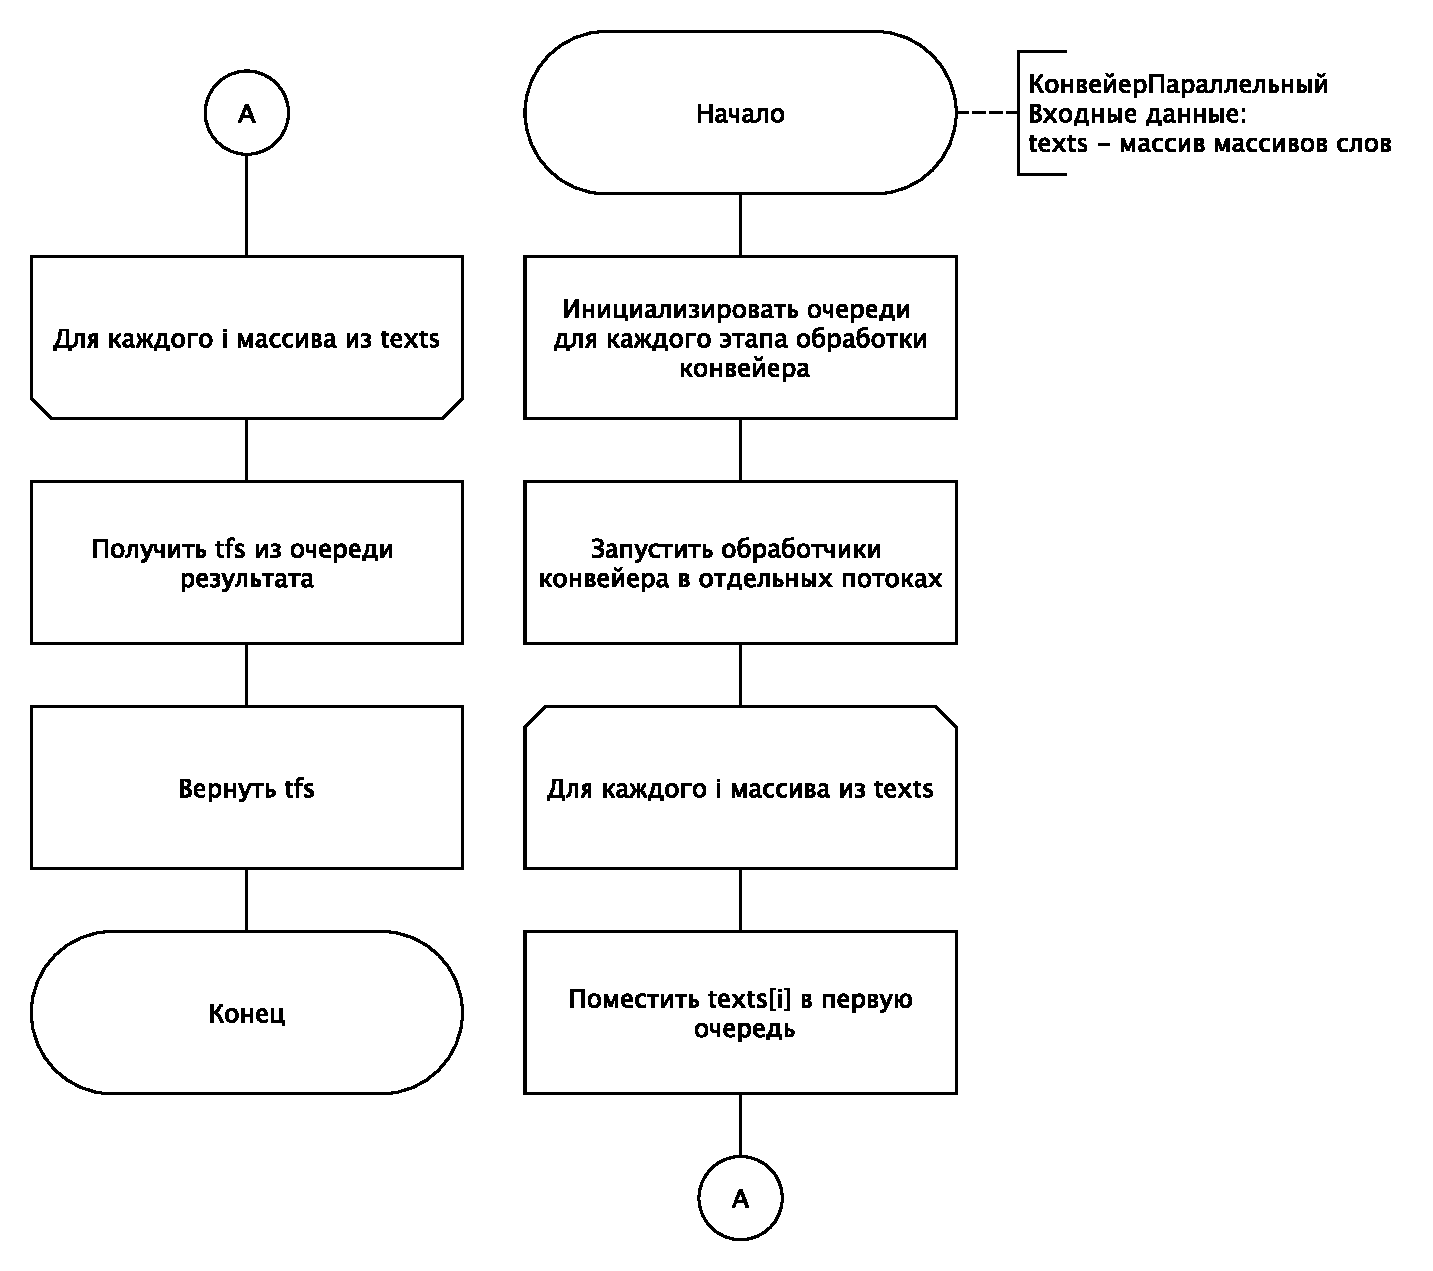
\includegraphics[width=0.6\linewidth]{pipeline_parallel.pdf}
    \caption{Схема алгоритма параллельной конвейерной обработки текста}
    \label{img:alg4}	
\end{figure}

\begin{figure}[h!]
\centering
    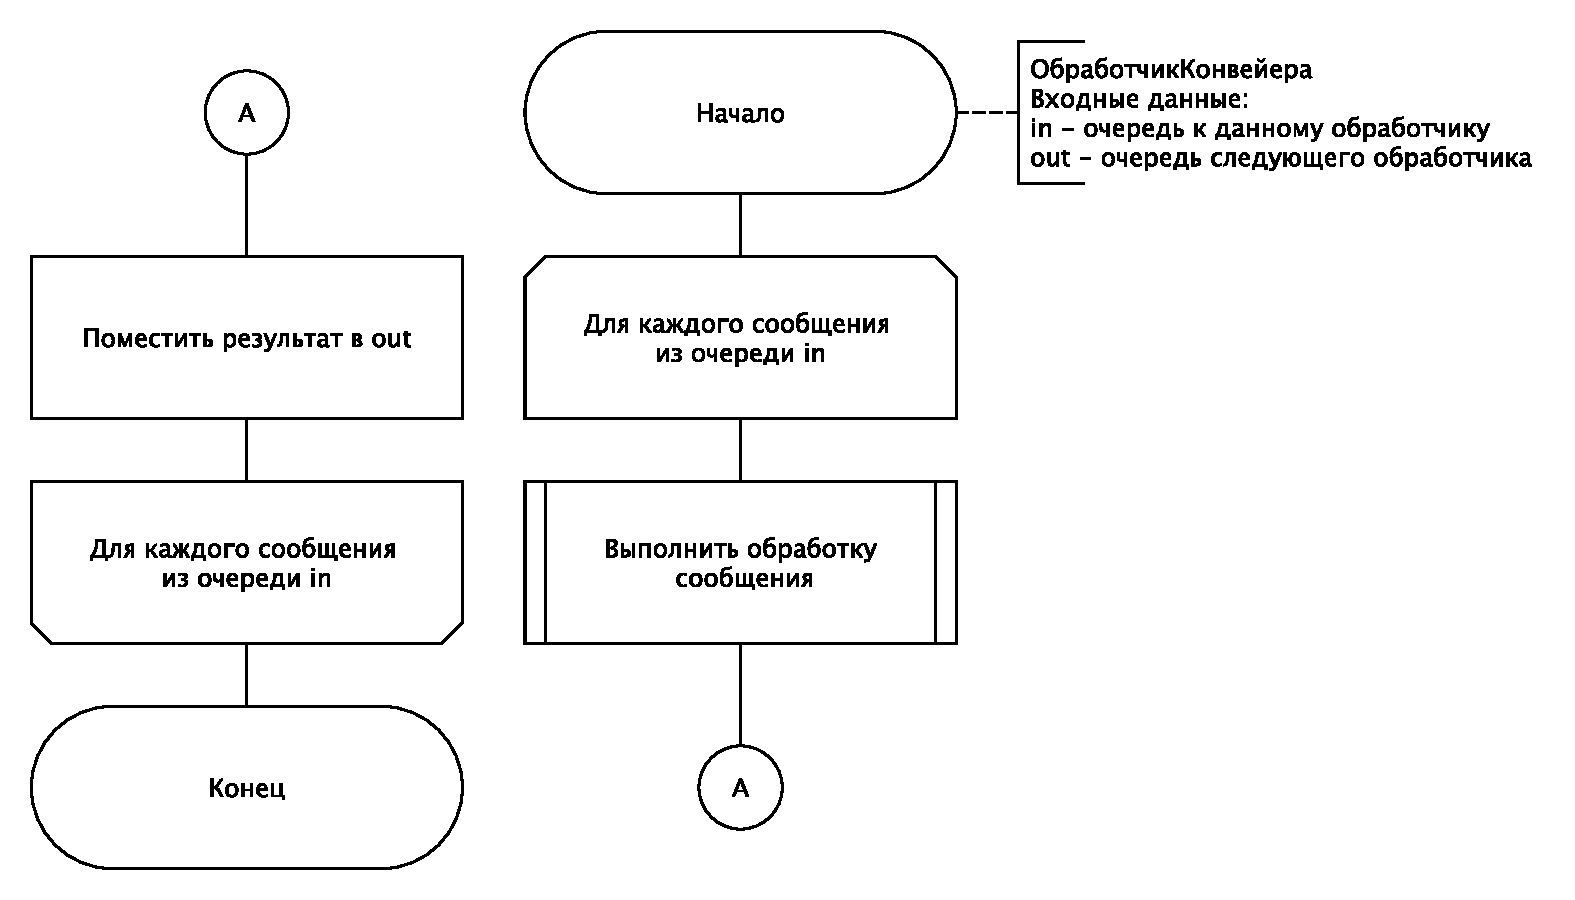
\includegraphics[width=0.7\linewidth]{pipeline_worker.pdf}
    \caption{Схема алгоритма обработчика конвейера}
    \label{img:alg5}	
\end{figure}

\newpage


\newpage